%%%%%%%%%%%%%%%%%%%%%%%%%%%%%%%%%%%%%%%%%
% Chemical Equations
% LaTeX Template
% Version 1.0 (14/10/12)
%
% This template has been downloaded from:
% http://www.LaTeXTemplates.com
%
% Original author:
% Martin Hensel (from the mhchem package documentation)
%
% License:
% CC BY-NC-SA 3.0 (http://creativecommons.org/licenses/by-nc-sa/3.0/)
%
% Note: to use these chemistry equations in your own document you will
% need to copy the \usepackage[version=3]{mhchem} line and paste it 
% before \begin{document} in your document. After this you can use the
% chemistry equation notation as exemplified in this document anywhere
% in your document.
%
%%%%%%%%%%%%%%%%%%%%%%%%%%%%%%%%%%%%%%%%%

\documentclass{article}

\usepackage[version=3]{mhchem} % Package for chemical equation typesetting
\usepackage{amsmath}
\usepackage[makeroom]{cancel}
\usepackage{physics}
\usepackage{tikz}
\usetikzlibrary{calc,scopes,angles,quotes,positioning}
\usepackage[portuges]{babel}
\usepackage{pdfpages}
%\usetikzlibrary{scopes}

\begin{document}
\everymath{\displaystyle}
\def\iangle{25} % Angle of the inclined plane

\def\down{-90}
\def\arcr{0.5cm} % Radius of the arc used to indicate angles


%									2a
\paragraph{2a)} ~\\

\begin{tikzpicture}[
    force/.style={>=latex,draw=blue,fill=blue},
    axis/.style={densely dashed,gray,font=\small},
    aux/.style={draw=gray,font=\small},
    M/.style={rectangle,draw,fill=lightgray,minimum size=0.5cm,thin},
    m/.style={rectangle,draw=black,fill=lightgray,minimum size=0.3cm,thin},
    plane/.style={draw=black,fill=blue!10},
    string/.style={draw=red, thick},
    pulley/.style={thick},
    tubo/.style={thick,draw=gray},
]


    %% Free body diagram of M
    \begin{scope}[rotate=\iangle]
        \node[M,transform shape] (M) {};
        \draw[tubo] (-2,-0.3) coordinate (base)
                     -- (2,-0.3);
	\draw[tubo] (2,+0.3) -- (-2,+0.3);
                     
        % Draw axes and help lines

        {[axis,->]
            \draw (0,-1.5) -- (0,1) node[right] {$\vec{n}$};
            \draw (-2,0) -- (2,0) node[right] {$tan$};
            
             
            % Indicate angle. The code is a bit awkward.


%            \draw[solid,shorten >=0.5pt] (\down-\iangle:\arcr)
%                arc(\down-\iangle:\down:\arcr);
%            \node at (\down-0.5*\iangle:1.3*\arcr) {$\phi$};
%            \draw[solid,shorten >=0.5pt] (\down-\iangle:\arcr*2)
%                arc(\down-\iangle:-180:\arcr*2);
%            \node at (\down-2*\iangle:1.3*\arcr*2) {$\alpha$};

        }
        {[axis]
         \draw (0,-2*tan{\iangle}) -- (-2,0);
	}
	{[aux]
	\draw (-1.5,0) arc (0:-\iangle:\arcr);
	\node at (-1.35,-0.175) {$\phi$};
	}

        % Forces
        {[force,->]
            % Assuming that Mg = 1. The normal force will therefore be cos(alpha)
            %\draw (M.center) -- ++(0,{cos(\iangle)}) node[above right] {$N$};
            \draw (M.west) -- ++(-1,0) node[above left=0.15cm] {$F_{gtan}$};
            %\draw (M.east) -- ++(1,0) node[above right] {$T$};
        }

    \end{scope}
    % Draw gravity force. The code is put outside the rotated
    % scope for simplicity. No need to do any angle calculations. 
    \draw[force,->] (M.center) -- ++(0,-1) node[below right=-0.15cm] {$F_g$};
    
    %%

\\

\end{tikzpicture}
\\
% first column
\begin{minipage}[t]{0.6\textwidth}
$
\\
m=0,5kg  \quad \phi = 25^\circ \\
F_g=mg\\
F_{gtan}=F_g \sin(\phi)=mg\sin(\phi)\\
\\
F=ma \Leftrightarrow a=\frac{F}{m}=g\sin(\phi)\\
\\
x=\frac{1}{2}a t^{2}\\
\\
x=\frac{1}{2}g \sin(\phi) t^2 \Leftrightarrow \frac{h}{\sin(\phi)}=\frac{1}{2}g\sin(\phi)t^2\\
\\
\Leftrightarrow \boxed{t=\sqrt{\frac{2h}{g\sin^2(\phi)}}=0.585s}\\
\\
%Alternativamente:\\
%\Delta T=\Delta V
%\Leftrightarrow mgh=\frac{1}{2}mv^2 \Leftrightarrow v=\sqrt{2gh}\\
%\\
%v=at \Leftrightarrow t=\frac{\sqrt{2gh}}{g\sin(\phi)}
$
%
%$V=-mgl \cos (\theta)$\\
%\\
%$T=\frac{1}{2}mv^{2}=\frac{1}{2}ml^2 \dot \theta^2$\\
%\\
%\boxed{L=\frac{1}{2}ml^2 \dot \theta^2+mgl \cos (\theta)}\\
%\\
%$
%\Rightarrow \frac{d}{dt} (ml^2 \dot \theta)=-mgl \sin (\theta)\\
%\\
%\Leftrightarrow \ddot \theta=-\frac{g}{l}\sin(\theta)$\\
%\\
%Para pequenos ângulos $\sin(\theta)\approx\theta\\
%\\
%\Rightarrow \ddot \theta=-\frac{g}{l}\theta \\
%\\
%\Leftrightarrow \theta=\sin(-\sqrt{\frac{g}{l}}t) \qquad \theta(t)=\sin(-\omega t)
%$
\end{minipage}
%second column
\begin{minipage}[t]{0.5\textwidth}
$
\Delta x \sin(\phi)=h\\
\Delta x=\frac{h}{\sin(\phi)}\\
$
%
%$v_k=\frac{\partial r_k}{\partial q_j}\dot q_j + \cancel{\frac{\partial r_k}{\partial t}}$\\
%\\
%$r(q,t)=(l\sin(\theta),l\cos(\theta))$\\
%\\
%$v=(l\dot \theta \cos(\theta), -l \dot \theta \sin(\theta)$
%
%$v^2=l^2 \dot \theta^2 \cancelto{1}{(\cos^2(\theta)+\sin^2(\theta))}$\\
%\\
%\\
%\\ \\ \\ \\ \\
%\boxed{\omega=\sqrt{\frac{g}{l}}}
\end{minipage}
\\
\\
\hrule
%%%%%%%%%%%%%%%%%%%%                     2b
\paragraph{2b)} ~\\
\\
$
F_{atr}=\mu F_{n}\\
\ddot r_{tan}=0 \Leftrightarrow F_{atr}=F_{gtan}\\
\\
F_n=mg\cos(\phi) \quad F_{gtan}=mg\sin(\phi)\\
\\
\boxed{\mu=\frac{\sin(\phi)}{\cos(\phi)}=tg(\phi)=0.466}\\
$
%2 graus de liberdade: $\theta$ e x\\
%\\
%$
%r_m=(x+l\sin(\theta),-l\cos(\theta)) \quad v_m=(\dot x+l\dot \theta \cos(\theta),l\dot \theta \sin(\theta)) \\
%\\
%v^2_m=(\dot x+l\dot \theta \cos(\theta))^2+(l\dot \theta \sin(\theta))^2=\dot x^2+2+\dot x+\dot \theta \cos(\theta)+l^2 \dot \theta^2 \cancelto{1}{(\cos^2(\theta)+\sin^2(\theta))}\\
%\\
%r_M=(x,cte) \quad v_M=\frac{\partial r_k}{\partial q_j} \dot q_j = (\dot x, 0) \qquad v^2_M=\dot x^2$ \\
%\\
%
%\boxed{L=\frac{M \dot x^2}{2}+\frac{m \dot x^2}{2}+m \dot xl \dot \theta \cos\theta+\frac{ml^2 \dot \theta^2}{2}+mgl\cos\theta}\\
\\
\hrule
 \pagebreak
%									2c
\paragraph{2c)} ~\\
\begin{tikzpicture}[
    force/.style={>=latex,draw=blue,fill=blue},
    axis/.style={densely dashed,gray,font=\small},
    aux/.style={draw=gray,font=\small},
    M/.style={rectangle,draw,fill=lightgray,minimum size=0.5cm,thin},
    m/.style={rectangle,draw=black,fill=lightgray,minimum size=0.3cm,thin},
    plane/.style={draw=black,fill=blue!10},
    string/.style={draw=red, thick},
    pulley/.style={thick},
    tubo/.style={thick,draw=gray},
]


    %% Free body diagram of M
    \begin{scope}[rotate=\iangle]
        \node[M,transform shape] (M) {};
        \draw[tubo] (-2,-0.3) coordinate (base)
                     -- (2,-0.3);
	\draw[tubo] (2,+0.3) -- (-2,+0.3);
                     
        % Draw axes and help lines

        {[axis,->]
            \draw (0,-1.5) -- (0,1) node[right] {$\vec{n}$};
            \draw (-2,0) -- (2,0) node[right] {$r$};
            
             
            % Indicate angle. The code is a bit awkward.


%            \draw[solid,shorten >=0.5pt] (\down-\iangle:\arcr)
%                arc(\down-\iangle:\down:\arcr);
%            \node at (\down-0.5*\iangle:1.3*\arcr) {$\phi$};
%            \draw[solid,shorten >=0.5pt] (\down-\iangle:\arcr*2)
%                arc(\down-\iangle:-180:\arcr*2);
%            \node at (\down-2*\iangle:1.3*\arcr*2) {$\alpha$};

        }
        {[axis]
         \draw (0,-2*tan{\iangle}) -- (-2,0);
	}
	{[aux]
	\draw (-1.5,0) arc (0:-\iangle:\arcr);
	\node at (-1.35,-0.175) {$\phi$};
	}

        % Forces
        {[force,->]
            % Assuming that Mg = 1. The normal force will therefore be cos(alpha)
            %\draw (M.center) -- ++(0,{cos(\iangle)}) node[above right] {$N$};
            \draw (M.west) -- ++(-1,0) node[above=0.32cm] {$F_{gtan}$};
            %\draw (M.east) -- ++(1,0) node[above right] {$T$};
        }

    \end{scope}
    % Draw gravity force. The code is put outside the rotated
    % scope for simplicity. No need to do any angle calculations. 
    \draw[force,->] (M.center) -- ++(0,-1) node[below right=-0.15cm] {$F_g$};
    {[axis]
    \draw (-1.81,-1.5) -- ++ (0,2.5) node[above=0.1cm]{$\omega$};
    %\node at (-1.35,-0.175) {$\phi$};
    \node at (-2,-1) {$r_0$};
    }
    \draw [aux,->](-1.5,1) arc (-70:-110:1) arc(250:110:0.05) arc (110:80:1);
    
    
    %%

\\

\end{tikzpicture}
\\
$
1 g.l. : r\\
\phi=25^\circ\\
\\
v_k=\frac{\partial r_k}{\partial q_j}\dot q_j + \frac{\partial r_k}{\partial t}\\
$
\begin{minipage}[t]{0.4\textwidth}
$
x=r\cos(\omega t)\cos(\theta)\\
y=r\sin(\omega t)\cos(\theta)\\
z=r\sin(\phi)\\
$
\end{minipage}
%second column
\begin{minipage}[t]{0.6\textwidth}
$
v_x=\dot{r}\cos(\omega t)\cos(\theta)-r\omega \sin(\omega t)\cos(\theta)\\
v_y=\dot{r}\sin(\omega t)\cos(\theta)-r\omega \cos(\omega t)\cos(\theta)\\
v_z=\dot{r}\sin(\phi)\\
$
\end{minipage}
$
\\
v^2=v.v=\dot{r}^2 \cos^2(\omega t)\cos^2(\phi)+r^2\omega^2 \sin^2(\omega t)\cos^2(\phi) +\dot{r}^2 \sin^2(\omega t)\cos^2(\phi)+r^2\omega^2 \cos^2(\omega t)\cos^2(\phi)
\cancel{-r\omega \sin(\omega t) \dot{r} \cos(\omega t)\cos^2(\phi)}\cancel{+r\omega \sin(\omega t) \dot{r} \cos(\omega t)\cos^2(\phi)}\\
\Leftrightarrow v^2=\dot{r}^2 \cos^2(\phi)(\cancelto{1}{\cos^2(\omega t)+\sin^2(\omega t))}+r^2 \omega^2 \cos^2(\phi)(\cancelto{1}{\cos^2(\omega t)+\sin^2(\omega t))}+\dot{r}^2 \sin^2 \phi\\
\\
L=T-V\\
V=mgr\sin(\phi)\qquad T=\frac{1}{2}m(\dot{r}^2\cos^2(\phi)+r^2\omega^2\cos^2(\phi)+\dot{r}^2\sin^2\phi)\\
\\
\dv{t} (\pdv{L}{\dot r})=\dv{t}(m\dot{r}\cos^2(\phi)+m\dot{r}\sin^2\phi)=\pdv{L}{r}=mr\omega^2-mg\sin\phi\\
\\
\Leftrightarrow m\ddot r=mr\omega^2-mg\sin\phi\\
\Leftrightarrow \boxed{\ddot r =r\omega^2-g\sin\phi}\\
$
%\dv{t} (\pdv{L}{\dot x})=$\boxed{M \ddot x + m \ddot x +ml\ddot \phi \cos \theta - ml\dot \theta^2 \sin \theta} $= \pdv{L}{x}=0 \\
%\\
%\dv{t} (\pdv{L}{\dot \theta})=\dv{t} (m\dot x l \cos \theta + ml^2 \dot \theta)=m\ddot xl\cos\theta-m\dot x l \dot \theta \sin \theta+ml^2 \ddot \theta\\
%\\
%\pdv{L}{\theta}=-m\dot xl\dot \theta \sin \theta - mgl\sin \theta\\
%\\
%\Rightarrow \ddot x\cos\theta\cancel{-\dot x \dot \theta \sin\theta}+l\ddot \theta=\cancel{-\dot x \dot \theta\sin\theta}-g\sin\theta \Leftrightarrow \ddot x\cos\theta+l\ddot\theta=-g\sin\theta\\
%r_{CM}=\frac{mr_m+Mr_m}{m+M}=\frac{(mx+ml\sin\theta,-ml\cos\theta)+(Mx,-MH)}{m+M}\\
%\\
%\dv[2]{r_{CM}}{t}=\frac{(\boxed{M \ddot x + m \ddot x +ml\ddot \theta \cos \theta - ml\dot \theta^2 \sin \theta},ml\ddot\theta\sin\theta+ml\dot\theta^2\cos\theta)}{m+M}\\
%\\
%\dv[2]{r_{CM}}{t}=(0,\frac{ml\ddot\theta\sin\theta+ml\dot\theta^2\cos\theta}{m+M})
%$
\hrule
%									2d
\paragraph{2d)} ~\\
$
\ddot r=0 \Leftrightarrow r\omega^2-g\sin\phi=0\\
\\
\boxed{\omega=\sqrt{\frac{g \sin \phi}{r}}}=6.436$ rad/s\\
\\
\hrule

\newpage

\includepdf[fitpaper=true, pages=2-3]{/home/halves/Dropbox/work/MOAero2019/scan.pdf}

%%									3a
%\paragraph{3a)} ~\\
%\\
%\begin{minipage}[t]{0.3\textwidth}
%$
%x_1=17t\\
%x_2=14-3t\\
%$
%\end{minipage}
%%second column
%\begin{minipage}[t]{0.3\textwidth}
%$
%\dot x_1=17\\
%\dot x_2=3\\
%$
%\end{minipage}
%\\
%$
%x_{CM}(t)=\frac{2\times 17t+5\times (3t+14)}{2+5}=7t+10 \qquad \dot x_{CM}=7 m/s\\
%$
%\\
%\hrule
%%									3b
%\paragraph{3b)} ~\\
%\\
%No ponto de compressão máxima $v_1=v_2=v_{CM}=7m/s\\
%\\
%\begin{minipage}[t]{0.6\textwidth}
%$
%T_i=\frac{1}{2}(2 \times 17^2+5 \times 3^2)=\frac{623}{2}\\
%\\
%T_{comp.max}=\frac{1}{2}(2+5)\times7^2=\frac{343}{2}\\
%$
%\end{minipage}
%\begin{minipage}[t]{0.3\textwidth}
%$
%T_i+\cancel{V_i}=T+V\\
%$
%\end{minipage}
%$
%\\
%$
%V=\frac{kx^2}{2}=T_i-T_{comp.max}\\
%\\
%\Leftrightarrow \frac{623}{2}-\frac{343}{2}=\frac{kx^2}{2} \Leftrightarrow x_{max}=\sqrt{\frac{280}{4480}}=0.25m\\
%$
%\\
%\hrule
%%									3c
%\paragraph{3c)} ~\\
%\\
%Trata-se duma colisão elástica e portanto $\Delta p =0$ e $\Delta E_c=0$:\\
%\\
%$2 \times 17+5\times3=2\times v_1+5 \times v_2 \Leftrightarrow v_1=\frac{49-5v_2}{2}\\$
%e\\
%$2 \times 17^2+5\times 3^2=2 \times v_1^2+5 \times v_2^2 \Leftrightarrow 623=(\frac{49-5v_2}{2})^2+5v_2^2 \\
%\\
%\Leftrightarrow 35v^2_ 2+490v_ 2+1155=0\\
%\\
%\Rightarrow v_ 2=\frac{490\pm 280}{70}=3 \vee \boxed{11} \Rightarrow v_1=17 \vee \boxed{-3}$
%
%

\end{document}